%\raggedbottom
%\chapter{Aplicaciones en VisualSLAM} \label{cap:aplicaciones}
\parskip=0pt
\section{Aplicaciones en VisualSLAM} \label{s:aplicaciones}

Hoy en día VisualSLAM ya tiene muchas aplicaciones y aún más que están por llegar en un futuro próximo, a continuación se expondrán varios ejemplos de aplicaciones, desde teléfonos móviles hasta robots aspiradora.

\subsection{Proyecto Tango}
El proyecto Tango es un proyecto colaborativo que trata de equipar a los smartphones y Tablets con sistema operativo Android la capacidad de medir la profundidad a la que se encuentra cada píxel de las imágenes capturadas por la cámara. Para ello los dispositivos compatibles con Tango dispondrán de 2 cámaras, una cámara RGB y otra que captura la profundidad, así el smartphone es capaz de construir un mapa en 3D del entorno (Figura \ref{fig:prototipoTango}. Los sensores del smartphone son capaces de tomar más de 250 millones de medidas 3D por segundo y con estos datos pueden  construir un modelo 3D de los alrededores del teléfono.
\begin{figure}[htbp]
\begin{center}
\subfigure[]{\label{fig:lenovo}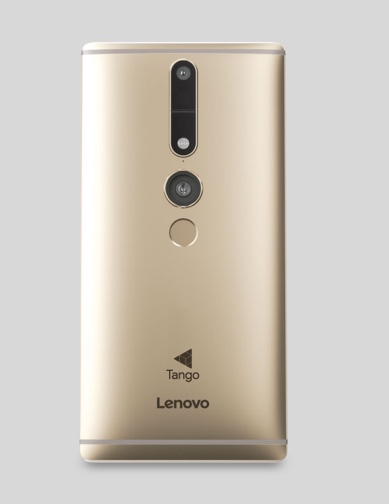
\includegraphics[height=4.5cm]{img/cap2/lenovo-phab2-pro.jpg}}
\hspace{0.5cm}
\subfigure[]{\label{fig:zenfone}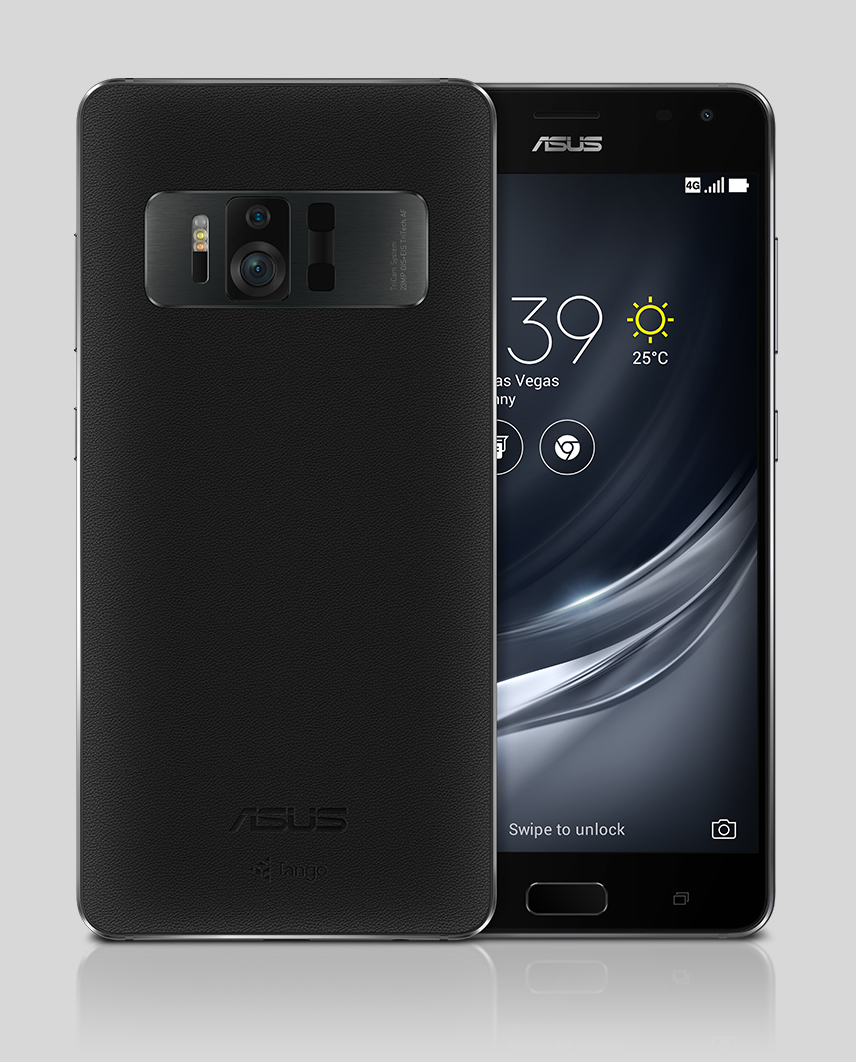
\includegraphics[height=4.5cm]{img/cap2/asus-zenfone-ar.jpg}}
\hspace{0.5cm}
\subfigure[]{\label{fig:prototipoTango}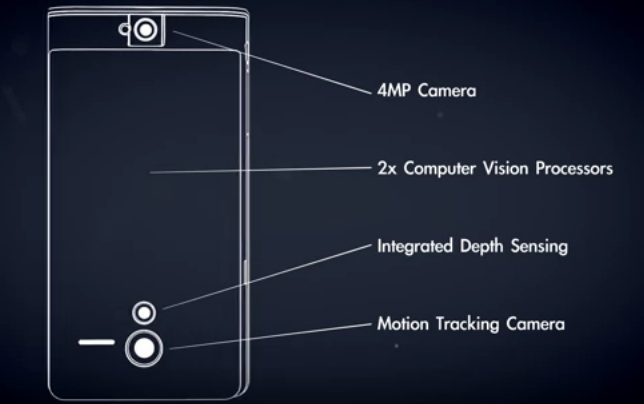
\includegraphics[height=4.5cm]{img/cap2/prototipo_Tango_smartPhone.png}}
\hspace{0.5cm}
\end{center}
\caption{El primer smartphone compatible con Tango de Lenovo(a). El primer Smartphone compatible con Tango y DayDream de ASUS (b).Esquema de prototipo de smartphone Tango (c).}
\end{figure}
Las posibilidades que ofrecerán este tipo de dispositivos serán muy variadas, desde medir las dimensiones de la habitación, hasta lo más útil como guiar a personas con discapacidades visuales en el interior de edificios. Pero también tendrá utilidades para el entretenimiento como convertir una habitación en el escenario de un juego mediante realidad aumentada.

Al ser una tecnología nueva aún no hay un elevado número de dispositivos que lo soporten. De momento existen 2 móviles compatibles con Tango \footnote{https://get.google.com/tango/}, el Lenovo  Phab 2 pro (Figura \ref{fig:lenovo}) y el Asus Zenfone AR (Figura \ref{fig:zenfone}).
En el caso del Zenfone AR  estará equipado con 3 cámaras traseras, una para seguir objetos (motion tracking), otra para detectar profundidad y otra de alta resolución de 23 MP.
Con estas 3 cámaras el smartphone podrá crear una modelo tridimensional del entorno y seguir su movimiento. La cámara de localización permitirá al ZenFone conocer su posición 3D en todo momento mientras se mueve por el entorno. La cámara de profundidad está equipada con un proyector de Infrarrojos que le permite medir distancias hasta los objetos en el mundo real.

\begin{figure}[htbp]
\begin{center}
\subfigure[]{\label{fig:mapaTango}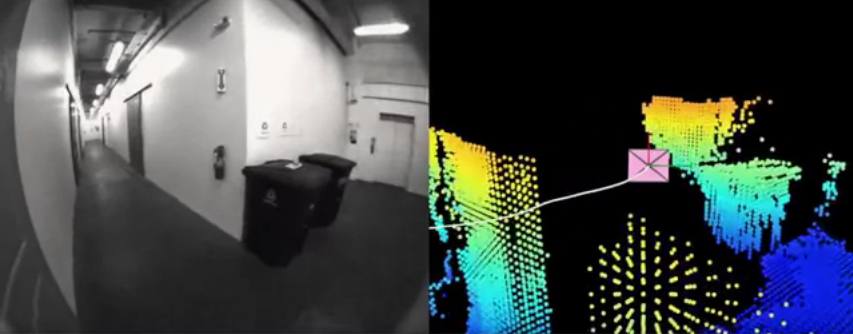
\includegraphics[height=3.0cm]{img/cap2/Proyecto_Tango_genera_mapa.png}}
\hspace{0.5cm}
\subfigure[]{\label{fig:makingMapTango}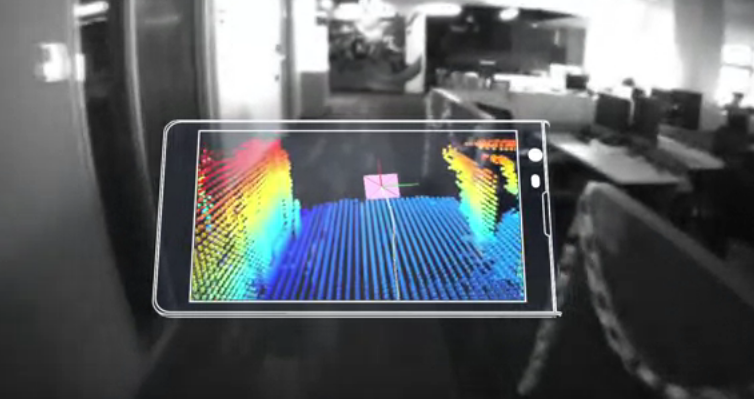
\includegraphics[height=3.0cm]{img/cap2/tangoDeviceMakingMap.png}}
\end{center}
\caption{Generación de mapa 1 (d). Generación de mapa 2 (e)}
\end{figure}

\clearpage

\subsection{Magic Plan}
Magic Plan es una aplicación que permite de forma interactiva obtener planos de habitaciones o del interior de un edificio, utilizando para ello la cámara de nuestra tablet o smartphone, sólo es necesario sacar fotos. Esta aplicación es gratuita, aunque si se desea obtener el plano en formato digital (pdf, jpg, csv y otros) será necesario pagar una pequeña cantidad de dinero.
Es muy sencilla de utilizar y en cuestión de minutos se obtiene un plano fiable (Figura \ref{fig:magicPlan}) sin necesidad de medir, dibujar, mover muebles  y sin necesidad de ser un experto.
La aplicación utiliza técnicas de VisualSLAM y se apoya también en la información de los giroscopios de los dispositivos. Es compatible con Android y dispositivos Apple.

En el caso de Android, actualmente la última versión es compatible con el sistema Tango, por tanto el procedimiento de captura es mucho más sencillo, robusto y preciso  ya que  permite detectar con mayor exactitud todas las paredes de la habitación, visualizarlas en 3D y aplicar realidad aumentada.

\begin{figure}[htbp]
\begin{center}
\subfigure[]{\label{fig:magicPlan}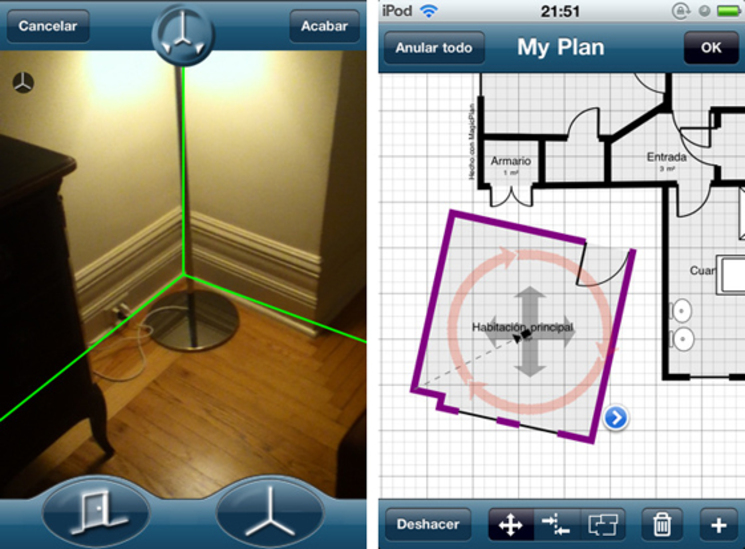
\includegraphics[height=8.0cm]{img/cap2/MagicPlan.jpg}}
\end{center}
\caption{La pantalla de un smartphone utilizando Magic Plan. }
\end{figure}
%\clearpage

\subsection{Pix4D}
Pix4D \footnote{https://pix4d.com/} es un software especializado en fotogrametría. Permite la posibilidad de generar mapas 2D y 3D desde fotografías. Las imágenes pueden ser transmitidas vía wireless a Pix4DDim para procesarlas y convertirlas a mapas 2D y 3D.  Posteriormente esta información será accesible desde la nube para poder analizarlas y compartirlas.
Pix4D permite crear mapas con exactitud a partir de fotografías de interiores, también tiene aplicaciones en minería para medir superficies y volúmenes (Figura \ref{fig:volumen}) de minas a cielo abierto, incluso se utiliza con finalidades forenses para recrear en 3D escenarios de accidentes, que posteriormente pueden ser analizadas con todo detalle.
También tiene aplicaciones en la agricultura para obtener mapas de cosechas utilizando la información que proporcionan las cámaras especiales como la Parrot Sequoia (Figura \ref{fig:parrotSequoia}).
Con la aplicación Pix4DCapture podremos controlar un dron desde nuestro smartphone para que genere un mapa. El dron puede volar de forma autónoma siguiendo algunas de las trayectoria de vuelo que trae por defecto el producto (Figura \ref{fig:dronTrayectoria}) o también puede generar el mapa mientras lo teledirigimos.

%\begin{figure}[htbp]
\begin{figure}[H]
\begin{center}
\subfigure[]{\label{fig:volumen}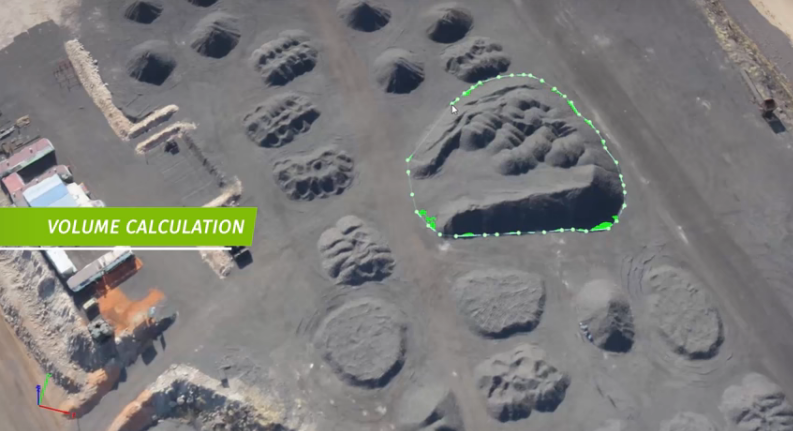
\includegraphics[height=3.0cm]{img/cap2/pix4d_volumen_calculo.png}}
\hspace{0.5cm}
\subfigure[]{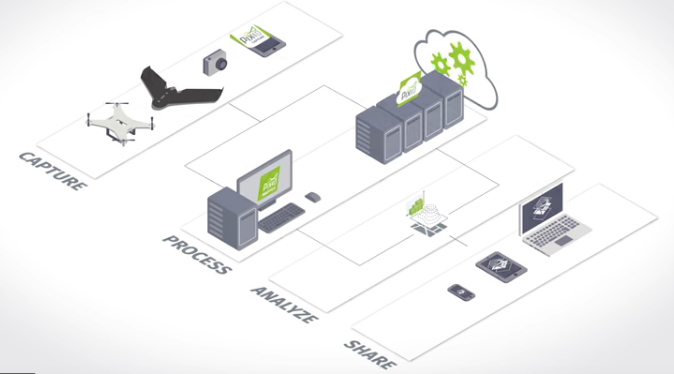
\includegraphics[height=3.0cm]{img/cap2/pix4d_esquema.png}}
\hspace{0.5cm}
\subfigure[]{\label{fig:dronTrayectoria}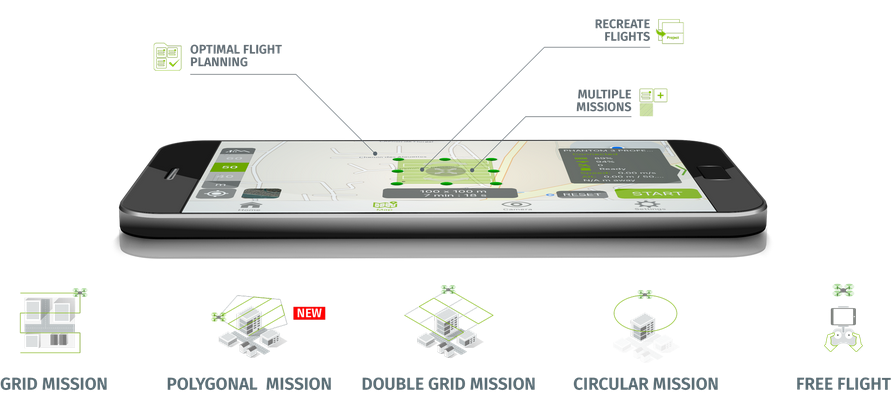
\includegraphics[height=4.0cm]{img/cap2/pix4d_dron_trayectorias.png}}
\hspace{0.5cm}
\subfigure[]{\label{fig:parrotSequoia}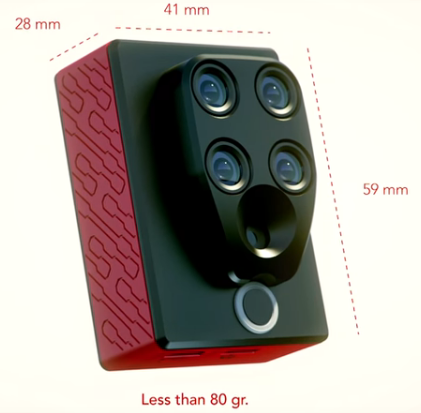
\includegraphics[height=4.0cm]{img/cap2/parrotSequoia.png}}
\end{center}
\caption{Pix4D cálculo de volumen(a). Flujo de datos de Pix4D(b). Trayectorias que pueden seguir los drones con Pix4DCapture(c). Cámara multiesprectral Parrot Sequoia (d)}
\end{figure}
%\clearpage

\subsection{Photo Tourism}
PhotoTourism o Photo Synth es un software inicialmente creado por la universidad de  Washington en colaboración con Microsoft. Es un sistema que toma grupos de conjuntos de fotografías disponibles online sobre un lugar en concreto, normalmente sobre un monumento turístico mundialmente conocido (como NotreDame, el Coliseo ( Figura \ref{fig:Coliseo}), La Fontana de Trevi) y es capaz de reconstruir puntos 3D de los monumentos y también calcular o estimar la posición de la cámara desde donde se tomaron las fotografías. Proporciona una nueva forma de navegar a través de fotografías de un destino turístico y una nueva forma de hacer visitas virtuales a monumentos.
Este sistema utiliza la técnica de \textit {Structure From Motion} SFM. SFM encuentra coincidencias de  puntos característicos entre distintas fotografías de un mismo lugar y que han sido tomadas desde distintos puntos de vista y así es capaz de calcular la localización 3D de dichos puntos característicos y también la localización 3D desde donde se tomaron las fotografías.
A diferencia de VisualSLAM, el procesamiento de estas fotografía es offline, sin necesidad de tiempo real, por lo que pueden ser ejecutadas desde un PC que por lo general tiene una capacidad de computación mucho mayor que una tablet o teléfono móvil.

\begin{figure}[htbp]
\begin{center}
\subfigure[]{\label{fig:Coliseo}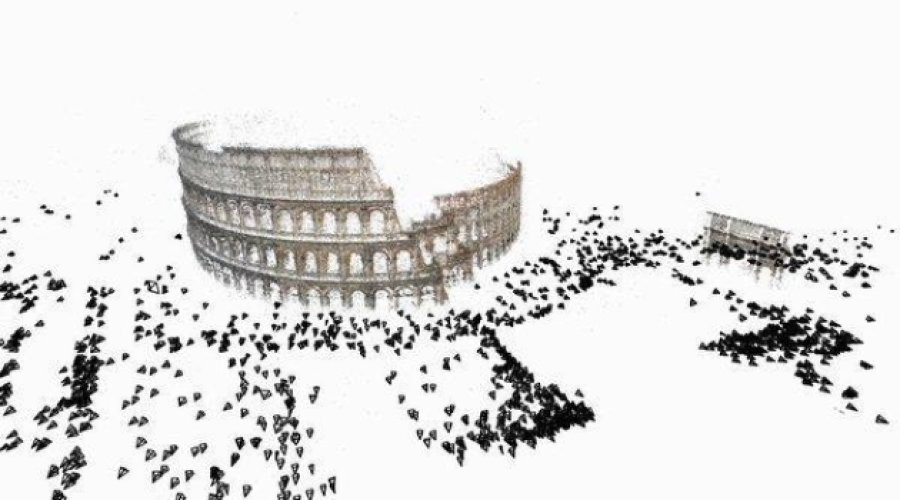
\includegraphics[height=8.0cm]{img/cap2/PhotoTourism.jpg}}
\end{center}
\caption{Recreación del Coliseo de Roma generado con Photo Tourism. }
\end{figure}
%\clearpage

\subsection{Canvas y el sensor Structure}
Canvas \footnote{https://canvas.io/ } es una herramienta de escaneo 3D enfocada a profesionales de la construcción o incluso aficionados al bricolaje en casa. La aplicación se ayuda del sensor de profundidad Structure. Este sensor se acopla en la parte trasera de un Ipad. Canvas permite obtener los planos en 3D de cualquier habitación de una manera fácil y sencilla, simplemente tendremos que pasear el Ipad equipado con el sensor Structure \footnote{https://structure.io/} alrededor de la habitación y podremos ver como el mapa 3D comienza a generarse en tiempo real. El sensor (Figura \ref{fig:Structure}) toma miles de medidas de profundidad que utilizará para generar el plano tridimensional. Los planos son almacenados en el Ipad y pueden ser consultados de manera interactiva posteriormente. Además permite que los planos generados sean convertidos a ficheros CAD.



\begin{figure}[htbp]
\begin{center}
\subfigure[]{\label{fig:Structure}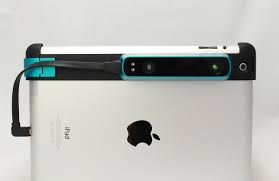
\includegraphics[height=5.0cm]{img/cap2/structureSensorCanvas.jpg}}
\end{center}
\caption{El sensor de profundidad Structure para Ipad. }
\end{figure}

%\clearpage

\subsection{Aplicaciones en Robótica Móvil}
Visual SLAM tiene aplicaciones directas en robótica. Un ejemplo podría ser el Robot Gita de Piaggio.
\begin {enumerate}
\item \textbf{El robot Gita}: Este novedoso robot ( Figura \ref{fig:gita} ) tiene incorporadas varios pares de cámaras estéreo, en la parte trasera y delantera. Con las imágenes captadas por estas cámaras se puede realizar VisualSLAM, además es capaz de seguir a su dueño siempre y cuando el humano lleve un cinturón con otras 2 cámaras estéreo, esta funcionalidad se consigue comparando el SLAM del robot con el SLAM captado por el cinturón.
El robot dispone de un compartimento interior o maletero y tiene suficiente potencia como para poder transportar hasta 20 Kg. Podría ser de gran utilidad a la hora de ir al supermercado, ya que el robot nos seguirá transportando la compra en su interior, no necesitaremos el típico carrito, incluso nos permitiría ir al centro comercial en bicicleta.

 Otra utilidad sería en el interior de un hotel, el robot podría realizar las funciones de camarero y hacer servicio de habitaciones transportando la comida directamente a las habitaciones del hotel. También podría ser un estupendo ayudante para un mecánico, ya que podría transportar la pesadas herramientas o piezas
\footnote{http://spectrum.ieee.org/automaton/robotics/home-robots/piaggio-cargo-robot}.


%\begin{figure}[htbp]
\begin{figure}[H]
\begin{center}
\subfigure[]{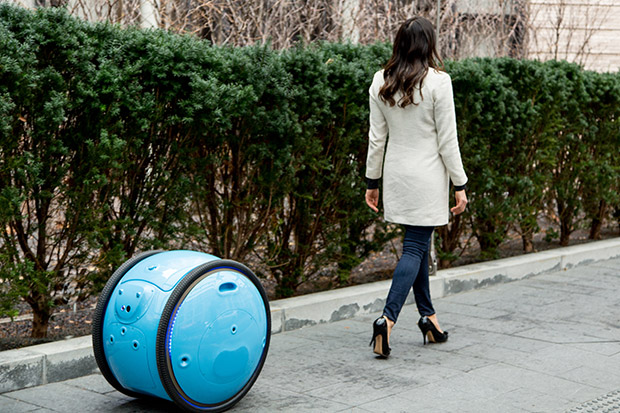
\includegraphics[height=6.0cm]{img/cap2/gita1.jpg}}
\hspace{0.5cm}
\subfigure[]{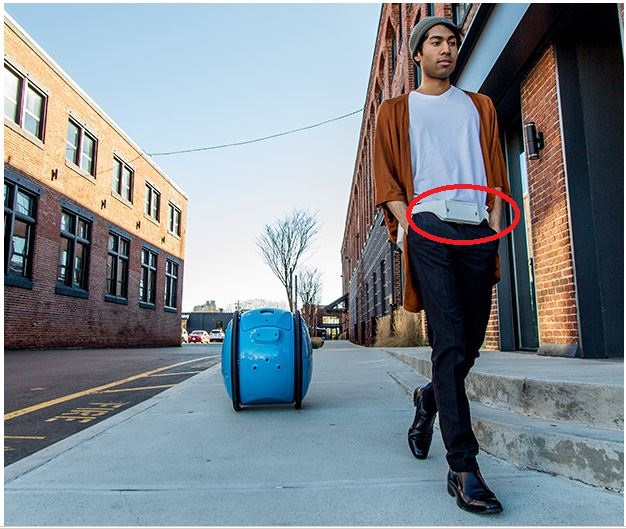
\includegraphics[height=6.0cm]{img/cap2/gita2.jpg}}
\hspace{0.5cm}
\subfigure[]{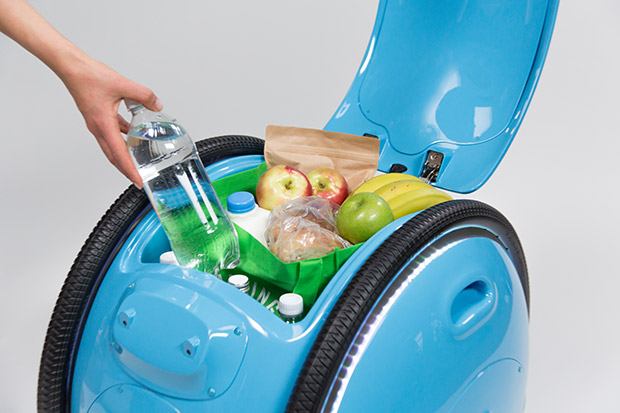
\includegraphics[height=5.5cm]{img/cap2/gita3.jpg}}
\end{center}
\caption{El Robot Gita siguiendo a su dueño (a) El cinturón con cámaras estéreo (b) La capacidad de carga del robot Gita (c)}
\label{fig:gita}
\end{figure}


\item \textbf{Reconocimiento de Objetos}: Otra utilidad de SLAM es que mejoran la capacidad de los robots móviles a la hora de reconocer objetos. Los sistemas de reconocimiento de objetos utilizarán la información proporcionada por SLAM para mejorar su capacidad de reconocimiento. La capacidad de reconocimiento será muy útil para aquellos robots que tengan que manipular objetos en su entorno. Con SLAM, los sistemas de reconocimiento pueden tomar como entradas varias imágenes desde distintos puntos de vista, por lo tanto el reconocimiento resulta más sencillo que si tuviesen tan sólo una imagen estática \footnote{http://www.roboticsproceedings.org/rss11/p34.pdf}.

\item \textbf{Robot Aspirador}: Recientemente ha entrado en los hogares el uso de VisualSLAM gracias a los últimos modelos de aspiradora equipados con cámaras.
Estos aspiradores robotizados disponen de cámaras que le permiten obtener un mapa de la habitación o planta del edificio y gracias a este mapa son capaces de aspirar toda la superficie del suelo de la habitación de manera eficiente, sin dejar ninguna zona de la planta sin limpiar.Además están equipados con sensores de proximidad, que les permiten esquivar obstáculos y aunque tengan que modificar su recorrido momentáneamente son capaces de seguir limpiando ya que pueden utilizar el mapa para continuar su ruta. Entre los distintos aspiradores estarían:
\begin{itemize}
\item Aspirador Dyson 360 Eye (Figura \ref{fig:Dyson})\footnote{http://www.dyson.come}.
\item Aspirador Roomba 966 (Figura \ref{fig:roomba})\footnote{http://www.irobot.es/robots-domesticos/aspiracion}.
\item Aspirador LG-Hombot (Figura \ref{fig:LG_hombot})\footnote{http://www.lg.com/es/aspiradoras/lg-VR64702LVMT}.
\end{itemize}

Tanto el modelo de Dyson como Roomba utilizan una cámara de 360 grados, 
en cambio el modelo de LG utiliza una doble cámara, y es capaz de aspirar la casa incluso en la oscuridad.

%\begin{figure}[htbp]
\begin{figure}[H]
\begin{center}
\subfigure[]{\label{fig:Dyson}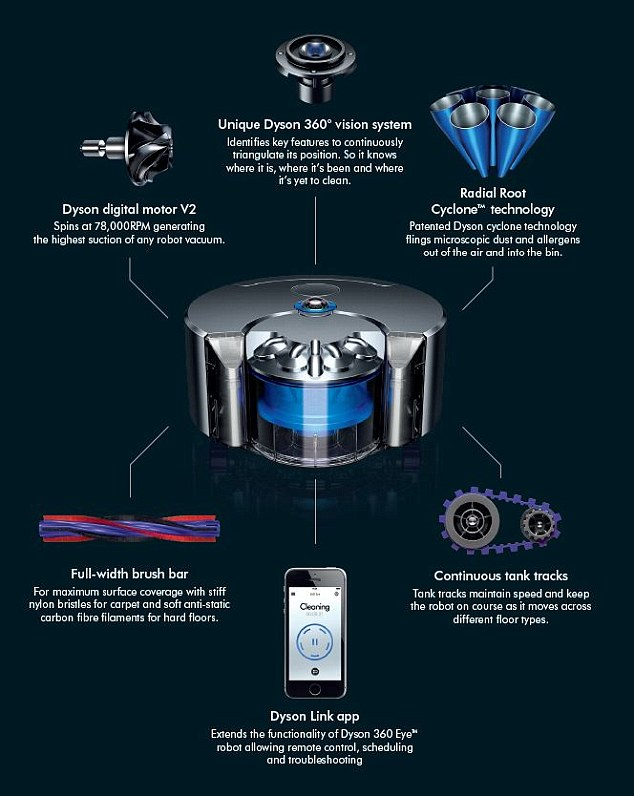
\includegraphics[height=6.0cm]{img/cap2/Dyson_360.jpg}}
\hspace{0.5cm}
\subfigure[]{\label{fig:roomba}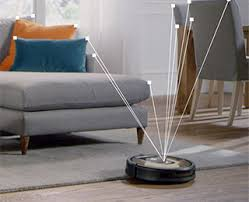
\includegraphics[height=6.0cm]{img/cap2/roomba_966.jpg}}
\hspace{0.5cm}
\subfigure[]{\label{fig:LG_hombot}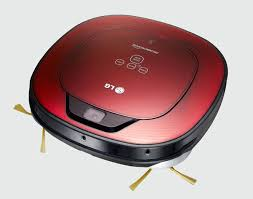
\includegraphics[height=6.0cm]{img/cap2/LG_hombot.jpg}}
\end{center}
\caption{Robot Dyson 360 Eye (a) Robot Roomba 966 (b) Robot Hombot de LG (c).}
\end{figure}

\item \textbf{Drones}: 
Por último no podemos olvidar los drones, robots voladores equipados con cámara que también pueden obtener mapas de su entorno con VisualSLAM. Existen también proyectos para equipar a drones con dispositivos compatibles con Tango para que sean capaces de obtener mapas de interiores con mayor precisión, robustez y velocidad \footnote{http://spectrum.ieee.org/automaton/robotics/drones/autonomous-quadrotor-flight-based-on-google-project-tango}.


%\begin{figure}[htbp]
\begin{figure}[H]
\begin{center}
\subfigure[]{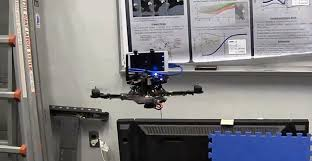
\includegraphics[height=5.0cm]{img/cap2/droneTango.jpg}}
\end{center}
\caption{Dron equipado con dispositivo compatible con Tango}
\end{figure}

\end {enumerate}





